\documentclass{standalone}

\usepackage{hyperref}
\usepackage{tikz}

\usetikzlibrary{decorations.pathreplacing,
  arrows,
  calc,
  decorations.pathmorphing,
  decorations.pathreplacing,
  decorations.markings,
  positioning,
  shapes,
  3d
}

\tikzstyle{snakearrow} = [decorate, decoration={pre length=0.2cm,
  post length=0.2cm, snake, amplitude=.4mm,
  segment length=2mm},thick, ->]

\ifpdf
  % Ensure reproducible output
  \pdfinfoomitdate=1
  \pdfsuppressptexinfo=-1
  \pdftrailerid{}
  \hypersetup{
    pdfcreator={},
    pdfproducer={}
  }
\fi

\def\statewidth{0.7}
\def\stategap{0.2}

\begin{document}
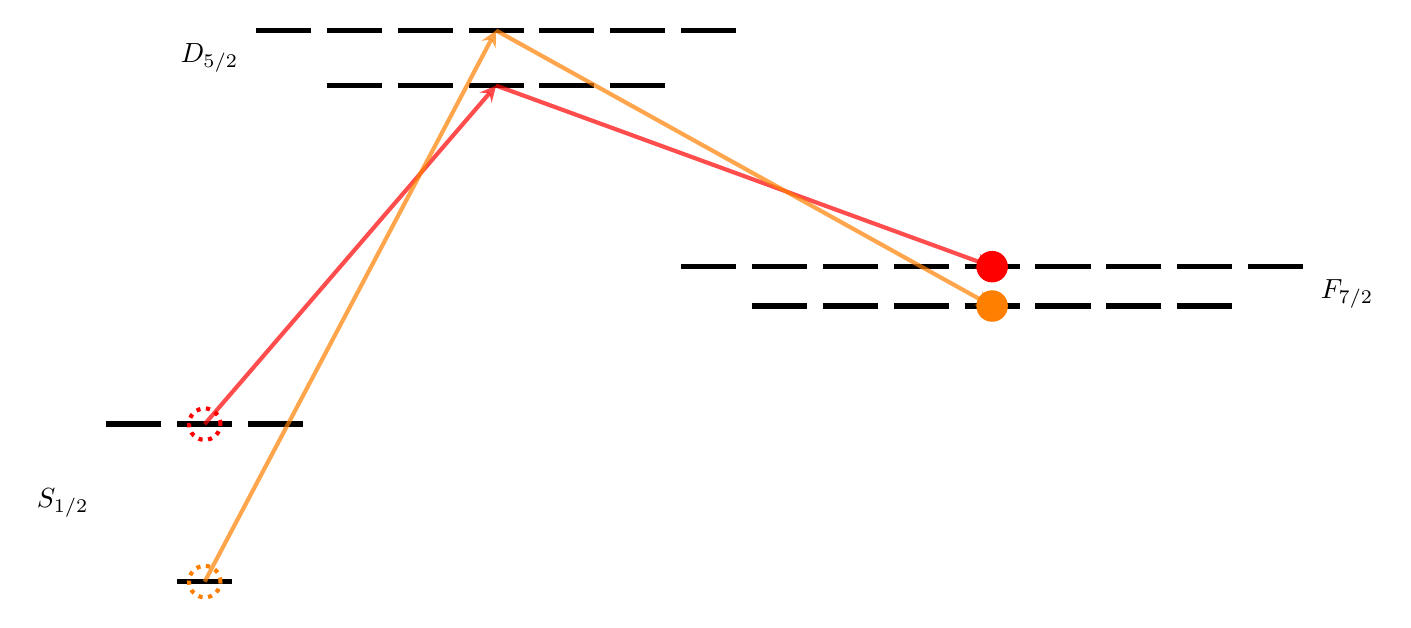
\begin{tikzpicture}
  % S 1/2
  \begin{scope}
    \draw[line width=2] ({\statewidth*-1.5-\stategap}, 0) -- coordinate (S1m1) ({\statewidth*-0.5-\stategap}, 0);
    \draw[line width=2] ({\statewidth*-0.5}, 0) -- coordinate (S10) ({\statewidth*0.5}, 0);
    \draw[line width=2] ({\statewidth*0.5+\stategap}, 0) -- coordinate (S11) ({\statewidth*1.5+\stategap}, 0);

    \node[left] at ({\statewidth*-1.5-\stategap-0.1}, -1) {$S_{1/2}$};

    \draw[line width=2] ({\statewidth*-0.5}, -2) -- coordinate (S00) ({\statewidth*0.5}, -2);
  \end{scope}

  % D 5/2
  \begin{scope}[shift={(3.7, 5)}]
    \draw[line width=2] ({\statewidth*-3.5-\stategap*3}, 0) -- coordinate (D3m3) ({\statewidth*-2.5-\stategap*3}, 0);
    \draw[line width=2] ({\statewidth*-2.5-\stategap*2}, 0) -- coordinate (D3m2) ({\statewidth*-1.5-\stategap*2}, 0);
    \draw[line width=2] ({\statewidth*-1.5-\stategap}, 0) -- coordinate (D3m1) ({\statewidth*-0.5-\stategap}, 0);
    \draw[line width=2] ({\statewidth*-0.5}, 0) -- coordinate (D30) ({\statewidth*0.5}, 0);
    \draw[line width=2] ({\statewidth*0.5+\stategap}, 0) -- coordinate (D31) ({\statewidth*1.5+\stategap}, 0);
    \draw[line width=2] ({\statewidth*1.5+\stategap*2}, 0) -- coordinate (D32) ({\statewidth*2.5+\stategap*2}, 0);
    \draw[line width=2] ({\statewidth*2.5+\stategap*3}, 0) -- coordinate (D33) ({\statewidth*3.5+\stategap*3}, 0);

    \node[left] at ({-\statewidth*3.5-\stategap*3-0.1}, -0.35) {$D_{5/2}$};

    \draw[line width=2] ({\statewidth*-2.5-\stategap*2}, -0.7) -- coordinate (D2m2) ({\statewidth*-1.5-\stategap*2}, -0.7);
    \draw[line width=2] ({\statewidth*-1.5-\stategap}, -0.7) -- coordinate (D2m1) ({\statewidth*-0.5-\stategap}, -0.7);
    \draw[line width=2] ({\statewidth*-0.5}, -0.7) -- coordinate (D20) ({\statewidth*0.5}, -0.7);
    \draw[line width=2] ({\statewidth*0.5+\stategap}, -0.7) -- coordinate (D21) ({\statewidth*1.5+\stategap}, -0.7);
    \draw[line width=2] ({\statewidth*1.5+\stategap*2}, -0.7) -- coordinate (D22) ({\statewidth*2.5+\stategap*2}, -0.7);
  \end{scope}

  % F 7/2
  \begin{scope}[shift={(10, 2)}]
    \draw[line width=2] ({\statewidth*-4.5-\stategap*4}, 0) -- coordinate (F4m4) ({\statewidth*-3.5-\stategap*4}, 0);
    \draw[line width=2] ({\statewidth*-3.5-\stategap*3}, 0) -- coordinate (F4m3) ({\statewidth*-2.5-\stategap*3}, 0);
    \draw[line width=2] ({\statewidth*-2.5-\stategap*2}, 0) -- coordinate (F4m2) ({\statewidth*-1.5-\stategap*2}, 0);
    \draw[line width=2] ({\statewidth*-1.5-\stategap}, 0) -- coordinate (F4m1) ({\statewidth*-0.5-\stategap}, 0);
    \draw[line width=2] ({\statewidth*-0.5}, 0) -- coordinate (F40) ({\statewidth*0.5}, 0);
    \draw[line width=2] ({\statewidth*0.5+\stategap}, 0) -- coordinate (F41) ({\statewidth*1.5+\stategap}, 0);
    \draw[line width=2] ({\statewidth*1.5+\stategap*2}, 0) -- coordinate (F42) ({\statewidth*2.5+\stategap*2}, 0);
    \draw[line width=2] ({\statewidth*2.5+\stategap*3}, 0) -- coordinate (F43) ({\statewidth*3.5+\stategap*3}, 0);
    \draw[line width=2] ({\statewidth*3.5+\stategap*4}, 0) -- coordinate (F44) ({\statewidth*4.5+\stategap*4}, 0);

    \node[right] at ({\statewidth*4.5+\stategap*4+0.1}, -0.35) {$F_{7/2}$};

    \draw[line width=2] ({\statewidth*-3.5-\stategap*3}, -0.5) -- coordinate (F3m3) ({\statewidth*-2.5-\stategap*3}, -0.5);
    \draw[line width=2] ({\statewidth*-2.5-\stategap*2}, -0.5) -- coordinate (F3m2) ({\statewidth*-1.5-\stategap*2}, -0.5);
    \draw[line width=2] ({\statewidth*-1.5-\stategap}, -0.5) -- coordinate (F3m1) ({\statewidth*-0.5-\stategap}, -0.5);
    \draw[line width=2] ({\statewidth*-0.5}, -0.5) -- coordinate (F30) ({\statewidth*0.5}, -0.5);
    \draw[line width=2] ({\statewidth*0.5+\stategap}, -0.5) -- coordinate (F31) ({\statewidth*1.5+\stategap}, -0.5);
    \draw[line width=2] ({\statewidth*1.5+\stategap*2}, -0.5) -- coordinate (F32) ({\statewidth*2.5+\stategap*2}, -0.5);
    \draw[line width=2] ({\statewidth*2.5+\stategap*3}, -0.5) -- coordinate (F33) ({\statewidth*3.5+\stategap*3}, -0.5);
  \end{scope}

  \draw[dotted,red, line width=1.5] (S10) circle (0.2);
  \draw[dotted,orange, line width=1.5] (S00) circle (0.2);

  \fill[red] (F40) circle (0.2);
  \fill[orange] (F30) circle (0.2);

  \draw[->, >=stealth, red, opacity=0.7, line width=1.5] (S10) -- (D20);
  \draw[->, >=stealth, red, opacity=0.7, line width=1.5] (D20) -- (F40);

  \draw[->, >=stealth, orange, opacity=0.7, line width=1.5] (S00) -- (D30);
  \draw[->, >=stealth, orange, opacity=0.7, line width=1.5] (D30) -- (F30);
\end{tikzpicture}
\end{document}
